\documentclass{article}
\usepackage{amsmath}
\usepackage{amsfonts}
\usepackage{amsthm}
\usepackage{amssymb}
\usepackage{tikz}
\usepackage{cleveref}

\newtheorem{lemma}{Lemma}
\newtheorem{theorem}{Theorem}
\newtheorem{observation}{Observation}

\begin{document}

\input{multi-fog-basic-formulation}

\section{\textcolor{red}{From here on this seems to be old and is now considered as archived}}

\section*{Resource Allocation Problem in Fog Computing}

\subsection*{Resource Graph}

\begin{figure}[h]
    \centering
    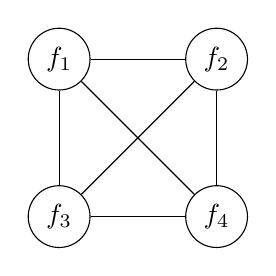
\begin{tikzpicture}
        % Nodes
        \node[draw, circle] (f1) at (0, 2) {$f_1$};
        \node[draw, circle] (f2) at (2, 2) {$f_2$};
        \node[draw, circle] (f3) at (0, 0) {$f_3$};
        \node[draw, circle] (f4) at (2, 0) {$f_4$};

        % Edges
        \draw (f1) -- (f2);
        \draw (f1) -- (f3);
        \draw (f1) -- (f4);
        \draw (f2) -- (f3);
        \draw (f2) -- (f4);
        \draw (f3) -- (f4);
    \end{tikzpicture}
    \caption{Resource Graph}
    \label{fig:resource_graph}
\end{figure}

\subsection*{Parameters}
\begin{itemize}
    \item $t_{if}$: Time to run task $i$ on fog node $f$
    \item $A_i$: Accuracy finishing task $i$
    \item $t_{\max}$: Max completion time
    \item $l_{if}$: Computational requirement of task $i$ on fog node $f$
    \item $d_{ij}$: Data volume to communicate from $T_i$ to $T_j$
    \item $b_{ff'}$: Bandwidth between fog nodes $f$ and $f'$
    \item $c_{ij}$: Time to communicate result from $T_i$ to $T_j$
    \item $t_i$: Computation time for task $T_i$
    \item $d_i$: Deadline for task $T_i$
\end{itemize}

\subsection*{Objective}
\begin{equation}
    \text{Maximize } \min \{x_i A_i\}
\end{equation}

\subsection*{Constraints}
\begin{equation}
    x_i \leq \max_j \{l_{ij}\}
\end{equation}

\begin{equation}
    t_i x_i + \max_{j \in I_i} \{y_j + c_{ji}\} \leq y_i \quad \text{for all } T_i
\end{equation}

\begin{equation}
    0 \leq y_i \leq d_i \quad \text{for all } T_i
\end{equation}

\begin{equation}
    0 \leq x_i \leq 1 \quad \text{for all } T_i
\end{equation}

\subsection*{Task Graph}

\begin{figure}[h]
    \centering
    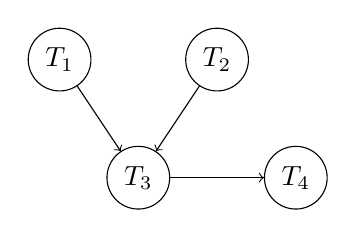
\begin{tikzpicture}
        % Nodes
        \node[draw, circle] (T1) at (0, 2) {$T_1$};
        \node[draw, circle] (T2) at (2, 2) {$T_2$};
        \node[draw, circle] (T3) at (1, 0.5) {$T_3$};
        \node[draw, circle] (T4) at (3, 0.5) {$T_4$};

        % Edges
        \draw[->] (T1) -- (T3);
        \draw[->] (T2) -- (T3);
        \draw[->] (T3) -- (T4);
    \end{tikzpicture}
    \caption{Task Graph}
    \label{fig:task_graph}
\end{figure}

\subsection*{Equations Specific to the Drawings}

For the resource graph:

\begin{itemize}
    \item Fog nodes: $f_1, f_2, f_3, f_4$
    \item Connections between fog nodes: $(f_1, f_2)$, $(f_1, f_3)$, $(f_1, f_4)$, $(f_2, f_3)$, $(f_2, f_4)$, $(f_3, f_4)$
\end{itemize}

For the task graph:

\begin{itemize}
    \item Tasks: $T_1, T_2, T_3, T_4$
    \item Dependencies: $T_1 \rightarrow T_3$, $T_2 \rightarrow T_3$, $T_3 \rightarrow T_4$
\end{itemize}

\subsection*{Variables and Equations}

\begin{itemize}
    \item $t_{i1}, t_{i2}, t_{i3}, t_{i4}$: Time to run task $i$ on fog nodes $f_1, f_2, f_3, f_4$
    \item $A_i$: Accuracy finishing task $i$
    \item $t_{\max}$: Max completion time
    \item $l_{i1}, l_{i2}, l_{i3}, l_{i4}$: Computational requirement of task $i$ on fog nodes $f_1, f_2, f_3, f_4$
    \item $d_{ij}$: Data volume to communicate from $T_i$ to $T_j$
    \item $b_{12}, b_{13}, b_{14}, b_{23}, b_{24}, b_{34}$: Bandwidth between fog nodes $f_1, f_2, f_3, f_4$
    \item $c_{13}, c_{23}, c_{34}$: Time to communicate result from $T_i$ to $T_j$
    \item $t_i$: Computation time for task $T_i$
    \item $d_i$: Deadline for task $T_i$
    \item $x_i$: Fraction of task $T_i$ executed
    \item $y_i$: Start time for task $T_i$
\end{itemize}

Constraints specific to the drawings:

\begin{equation}
    x_i \leq \max \{l_{i1}, l_{i2}, l_{i3}, l_{i4}\}
\end{equation}

\begin{equation}
    t_i x_i + \max_{j \in I_i} \{y_j + c_{ji}\} \leq y_i \quad \text{for all } T_i
\end{equation}

\begin{equation}
    0 \leq y_i \leq d_i \quad \text{for all } T_i
\end{equation}

\begin{equation}
    0 \leq x_i \leq 1 \quad \text{for all } T_i
\end{equation}

For the task dependencies:
\begin{equation}
    y_3 \geq y_1 + c_{13}
\end{equation}

\begin{equation}
    y_3 \geq y_2 + c_{23}
\end{equation}

\begin{equation}
    y_4 \geq y_3 + c_{34}
\end{equation}


\section{Multi-Fog Formulation}
\subsection{Tasks cannot be run in multiple fogs}
Assumptions: 
\begin{itemize}
    \item Tasks are not preemptive, i.e., a task cannot be started in one fog, stopped, moved to another fog, and continued.
    \item Tasks can be run in at most one fog
    \item A task can receive data from all in-neighbors simultaneously
\end{itemize}

\subsection*{Parameters}
\begin{itemize}
    \item $t_{if}$: Time to run $T_i$ on fog $f$
    \item $A_i$: Accuracy if $T_i$ is run completely
    \item $t_{\max}$: Max completion time
    \item $d_{ij}$: Data volume to communicate from $T_i$ to $T_j$
    \item \( b_{ff'} \): Bandwidth between fogs \( f \) and \( f' \) (in Hz).
    \item \( \text{SNR} \): Signal-to-noise ratio of the communication channel (dimensionless).
    \item \( c_{ij}^{f'f} \): Communication time between \( T_i \) and \( T_j \), where \(T_i\) is executed in fog\( f \) and \(T_i\) is executed in fog\( f' \), given by Shannon's equation: 
    \[
    c_{ij}^{f'f} = \frac{d_{ij}}{b_{ff'} \log_2(1 + \text{SNR})}
    \]
    \item $P_{if} \in \{0,1\}$ : Binary variable indicating if task i is permitted to be executed in fog $f$
\end{itemize}
\subsection*{Variables}
\begin{itemize}
    \item $l_{if} \in [0,1]$: Fraction of $T_{i}$ computed in fog $f$
    \item $e_{if} \in \{0,1\}$: Whether $T_{i}$ is executed in fog $f$
    %\item \( x_{if} \): Binary variable indicating the final assignment of task \( T_i \) to fog node \( f \) (1 if true, 0 otherwise).  
    \item $y_{i} \in [0,t_{\max}]$: Min time to complete $T_i$ across all fogs
    \item $z_{ji}^{f'f}\in \{0,1\}$: Binary variable introduced to linearize the product \( e_{if} \cdot e_{jf'} \)
    
\end{itemize}
\subsection*{Objective}
\begin{equation}
    \text{Maximize } \min_i \{A_i \sum_f l_{if} \} \label{eq:obj}
\end{equation}
\subsection*{Constraints}
\begin{align}
    l_{if} &\leq e_{if}, \forall i, f \label{eq:run-flag} \\ 
    M_i = \max_{j \in \text{in}_i} \left( y_j + \sum_{f, f'} z_{ji}^{f'f}  c_{ij}^{f'f} \right) \forall i, j, f, f'\\
    \sum_f t_{if} l_{if} + M_i \leq y_i, \quad \forall i \label{eq:time-rest} \\
    y_i &\leq t_{\max}, \forall i \\
    \sum_f e_{if} & \leq 1, \forall i \label{eq:one-fog} \\
    l_{if} \leq P_{if} \forall i,f \\
    z_{ji}^{f'f} &\leq e_{if}, \forall i, j, f, f' \label{eq:z-e-if} \\
    z_{ji}^{f'f} &\leq e_{jf'}, \quad \forall i, j, f, f' \label{eq:z-e-jf} \\
    z_{ji}^{f'f} &\geq e_{if} + e_{jf'} - 1, \forall i, j, f, f' \label{eq:z-linearization}\\
    M_i \geq y_j + \sum_{f, f'} z_{ji}^{f'f} \cdot c_{ij}^{f'f}, \quad \forall j \in \text{in}_i
\end{align}
Properties:
\begin{enumerate}
    \item From Eq.~\ref{eq:one-fog}, a task is executed in at most one fog.
    % \item From Eq.~\ref{eq:one-fog}, a task is finally assigned to exactly one fog node.
    \item From Bullet 1 and Eq.~\ref{eq:run-flag}, for each task $T_i$ at most one variable $l_{if}$ is larger than 0.
    \item From Bullet 2, in Eq.~\ref{eq:obj} it holds that $\sum_f l_{if} = \max_f \{l_{if}\}$
    \item From Bullet 2, in Eq.~\ref{eq:time-rest} at most one term of $\sum_f t_{if} l_{if}$ is different from 0.
    \item From Bullet 1, in Eq.~\ref{eq:time-rest} at most one term of $\sum_{f,f',j \in in_i} e_{if} e_{jf}  c_{ji}^{f'f}$ is different from 0 
    \item From Eq.~\ref{eq:z-e-if}, Eq.~\ref{eq:z-e-jf}, and Eq.~\ref{eq:z-linearization}, \( z_{ji}^{f'f} \) equals 1 if and only if both \( e_{if} \) and \( e_{jf'} \) are 1; otherwise, it equals 0.
\end{enumerate}

\section{Tasks can be run in multiple fogs}
Assumptions: 
\begin{itemize}
    \item Tasks are not preemptive, i.e., a task cannot be started in one fog, stopped, moved to another fog, and continued.
    \item Tasks can be run in several fogs.
    \item Accuracy is given by maximum fraction of a task run in any fog 
\end{itemize}

\subsection*{Parameters}
\begin{itemize}
    \item $t_{if}$: Time to run $T_i$ on fog $f$
    \item $A_i$: Accuracy if $T_i$ is run completely
    \item $t_{\max}$: Max completion time
    \item $d_{ij}$: Data volume to communicate from $T_i$ to $T_j$
    \item \( b_{ff'} \): Bandwidth between fogs \( f \) and \( f' \) (in Hz).
    \item \( \text{SNR} \): Signal-to-noise ratio of the communication channel (dimensionless).
    \item \( c_{ij}^{f'f} \): Communication time between \( T_i \) and \( T_j \), where \(T_i\) is executed in fog\( f \) and \(T_i\) is executed in fog\( f' \), given by Shannon's equation: 
    \[
    c_{ij}^{f'f} = \frac{d_{ij}}{b_{ff'} \log_2(1 + \text{SNR})}
    \]
\end{itemize}
\subsection*{Variables}
\begin{itemize}
    \item $l_{if} \in [0,1]$: Fraction of $T_{i}$ computed in fog $f$
    \item $e_{if} \in \{0,1\}$: Whether $T_{i}$ is executed in fog $f$
    \item $y_{i} \in [0,t_{\max}]$: Min time to complete $T_i$ across all fogs
    \item $z_{ji}^{f'f}\in \{0,1\}$: Binary variable introduced to linearize the product \( e_{if} \cdot e_{jf'} \)
\end{itemize}
\subsection*{Objective}
\begin{equation}
    \text{Maximize } \min_i \{A_i \max_f l_{if} \} \label{eq:obj2}
\end{equation}
\subsection*{Constraints}
\begin{align}
    l_{if} &\leq e_{if}, \forall i, f \label{eq:run-flag-multi} \\ 
    \sum_f e_{if} \geq 1, \forall i \label{eq:multi-fog-exact} \\  % Ensure the task can be executed in multiple fogs
    \sum_f t_{if} l_{if} + 
    \sum_{j \in in_i} y_j + 
    \sum_{f, f', j \in in_i} z_{ji}^{ff'} \cdot c_{ij}^{ff'} &\leq y_i, \quad \forall i \label{eq:time-rest-multi} \\
    y_i &\leq t_{\max}, \forall i \\
    z_{ji}^{ff'} &\leq e_{if}, \forall i, j, f, f' \label{eq:z-e-if-multi} \\
    z_{ji}^{ff'} &\leq e_{jf'}, \quad \forall i, j, f, f' \label{eq:z-e-jf-multi} \\
    z_{ji}^{ff'} &\geq e_{if} + e_{jf'} - 1, \forall i, j, f, f' \label{eq:z-linearization-multi} 
\end{align}



\end{document}
